Die bisherige Herangehensweise, den Niederschlag über das Jahresmittel zu Evaluieren. Ist nicht hinreichend genau. Da dadurch die lokale und vor allem zeitliche Varianz zu stark beeinträchtigt wird. Bezieht man hingegen das 99. Quantil der Daten wird die in \ref{sec:zusammenfassung_01} angesprochene tägliche Inkonsistenz umgangen. Das 99. Quantil der Niederschläge entspricht den stärksten örtlichen Regenereignissen. D. Maraun bespricht im Paper \cite{biasMaraun} eine Herangehensweise, in der auch noch die Daten zuvor in die Jahreszeiten aufgeteilt werden, da die Starkregen je nach Jahreszeit unterschiedlichst ausfallen und unterschiedliche Trigger-Mechanismen haben. Im diesem Kapitel wird zunächst aber das 99. Quantil des gesamten Jahres betrachtet, um einen Vergleichswert der stärksten Regenereignisse des gesamten Jahres zu erhalten.
\section{Herangehensweise}
\begin{itemize}
	\item Berechnung des 99. jährlichen Quantils aller Datensätze
	\item Vergleichen dieses Quantils mit dem Quantil der Beobachtungsdaten.
\end{itemize}

\section{Differenzen im 99. Quantil} \label{sec:diff_q99}
Von den Datensätzen (historical, evaluation und APGD) wurden zunächst das alljährliche 99. Quantil berechnet. In Folge wurde von den Modelldaten, wie bereits in Kapitel \ref{chap:mean}, die Beobachtungsdaten abgezogen. Da für den Datensatz Evaluation ALP-3, wie schon in Kapitel \ref{sec:zusammenfassung_01} erwähnt, am Rand des Datensatzes ein Gebiet großer Ausreißer herrschte, wurde dieses für eine bessere Darstellung ausgeschnitten und auch für die Erstellung des Boxplots ausgelassen. Da diese werte die normalen Abweichung überschatteten. Die unveränderten Abweichungen sind in der Abbildung \ref{fig:quantile_eval_alp3} dargestellt. Wie dort zu erkennen ist, verfälscht der Bereich auch den Bias der Abweichungen ins Positive.\\
Die Abbildungen \ref{fig:quantile_all_boxplots} weisen darauf hin, dass das regionale Konvektion-erlaubende Klimamodell CCLM5-0-9, betrieben mit Re-Analysedaten (Evaluation ALP-3), ein relativ gutes Ergebnis für Starkregenereignisse liefert. Betrachtet man den dazugehörigen Historical-Datensatz erkennt man, dass dieser im Vergleich mit dem Modell CCLM4-8-17 eine stärkerer mittlere Abweichung und größere Ausreißer liefert. Das könnte darauf hinweisen, dass das Modell CCLM5-0-9 sensibler auf falsche Daten reagiert (im Historical-Datensatz wurde das Modell mit den historischen Daten eines GCMs betrieben und bilden deshalb nicht immer den richtigen Zustand der Atmosphäre ab). Und es daher zu starken Fluktuationen kommt. Es könnte sich auch um ein aufgeschaukeltes Phänomen handeln, da CCLM5-0-9 in das gröbere Modell eingenested betrieben wurde. Die mir hier zur Verfügung stehenden Daten zu beiden Modellen reichen leider nicht aus, um eine sichere Aussage treffen zu können.\\

\begin{figure}[h]
	\begin{subfigure}{0.49\textwidth}
		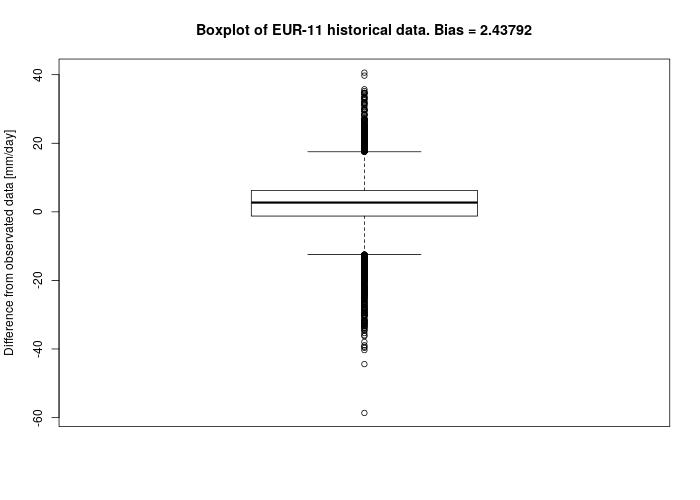
\includegraphics[width=\textwidth]{quantile_all/diff_q99_boxplot_hist_eur11.jpg}
		\caption{EUR-11, Historical}
	\end{subfigure}
	\begin{subfigure}{0.49\textwidth}
		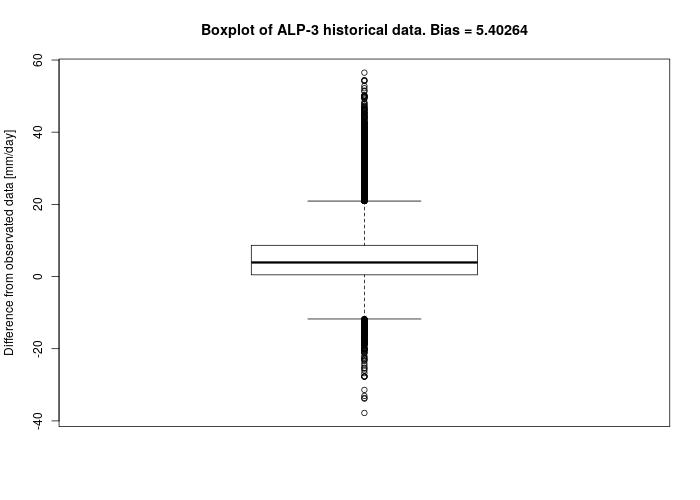
\includegraphics[width=\textwidth]{quantile_all/diff_q99_boxplot_hist_alp3.jpg}
		\caption{ALP-3, Historical}
	\end{subfigure}
	\begin{subfigure}{0.49\textwidth}
		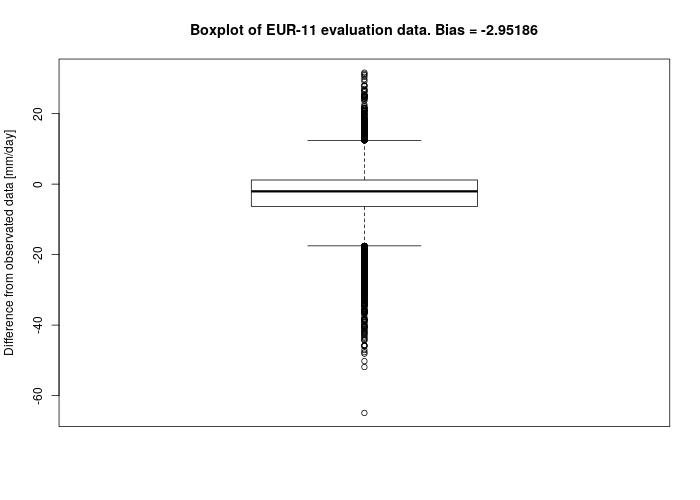
\includegraphics[width=\textwidth]{quantile_all/diff_q99_boxplot_eval_eur11.jpg}
		\caption{EUR-11, Evaluation}
	\end{subfigure}
	\begin{subfigure}{0.49\textwidth}
		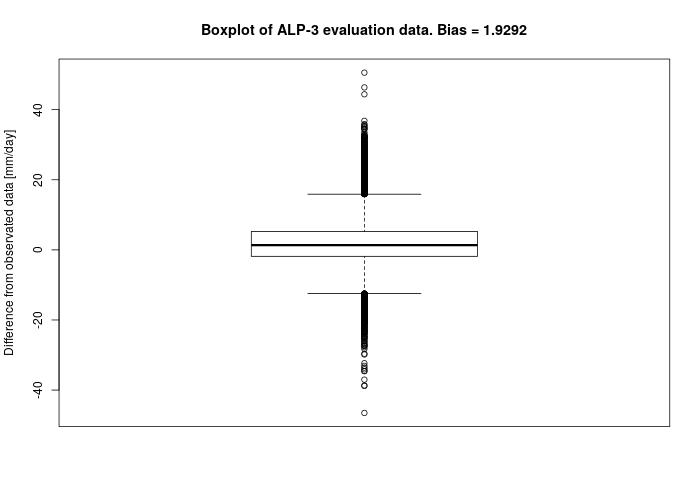
\includegraphics[width=\textwidth]{quantile_all/diff_q99_boxplot_eval_alp3.jpg}
		\caption{ALP-3, Evaluation}
	\end{subfigure}
	\caption{Boxplots der Abweichungen im 99. Quantil, aller Jahre für die 4 Datensätze. In Evaluation ALP-3 wurde, wie in Kapitel \ref{sec:diff_q99} beschrieben, ein Ausreißer-Bereich ausgeschnitten. Für die unveränderte Darstellung siehe Abb. \ref{fig:quantile_eval_alp3}.}
	\label{fig:quantile_all_boxplots}
\end{figure}

Die Grafiken von Abb.\ref{fig:quantile_all} geben Aufschluss darüber, wo die größten Abweichungen liegen. Beachtenswert ist, dass sich die größten Abweichungen nun auf drei Hauptspots reduzieren, welche im Südwesten des Alpenhauptkamms, bei Genua und an der Italienisch-Slowenischen Grenze, liegen. Dies gilt für alle Datensätze. Im Gegensatz zu den eher großräumigen Abweichungen im mittleren Niederschlag (vgl. Kapitel \ref{chap:mean}) sind diese sehr punktuell. Noch dazu ist auffallend, dass die beiden Datensätze des regionalen Klimamodells CCLM5-0-9 auf großen Gebieten die Starkregen gut abbilden und nur in einigen gebirgigen Gebieten den Regen stark über- bzw. unterschätzen. Was für ein mangelndes fein-tuning des Modells spricht, da genau diese Gebiete besonders herausfordernd für das Modell sind, im Schnitt das Modell aber gute Ergebnisse liefert.\\


\begin{figure}
	\begin{subfigure}{0.49\textwidth}
		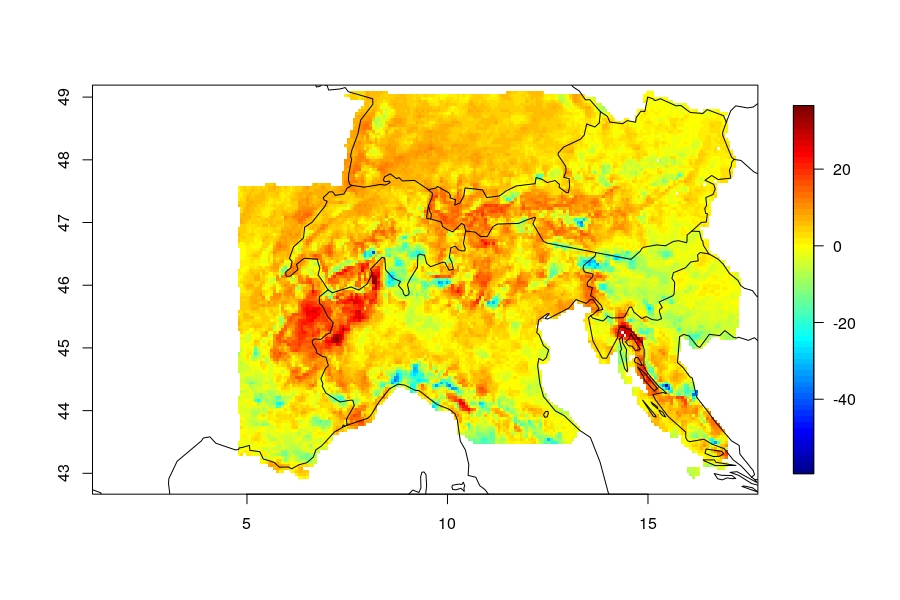
\includegraphics[width=\textwidth]{quantile_all/diff_q99_hist_eur11.jpeg}
		\caption{EUR-11, Historical}
	\end{subfigure}
	\begin{subfigure}{0.49\textwidth}
		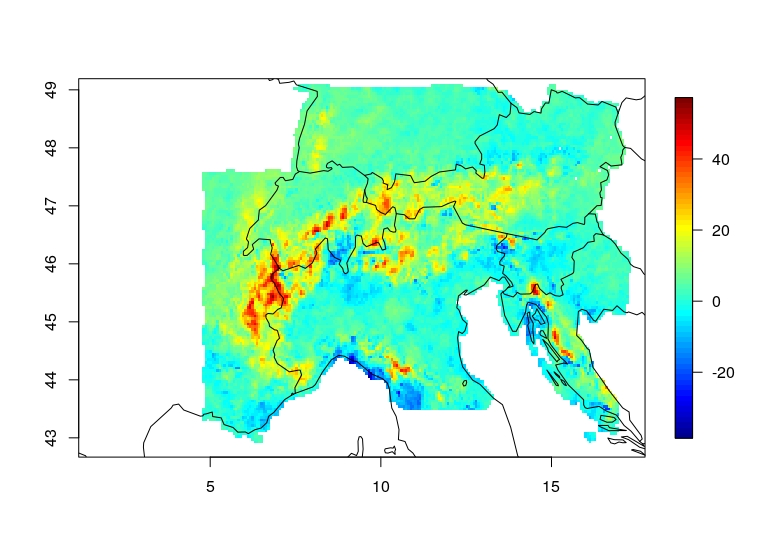
\includegraphics[width=\textwidth]{quantile_all/diff_q99_hist_alp3.jpeg}
		\caption{ALP-3, Historical}
	\end{subfigure}
	\begin{subfigure}{0.49\textwidth}
		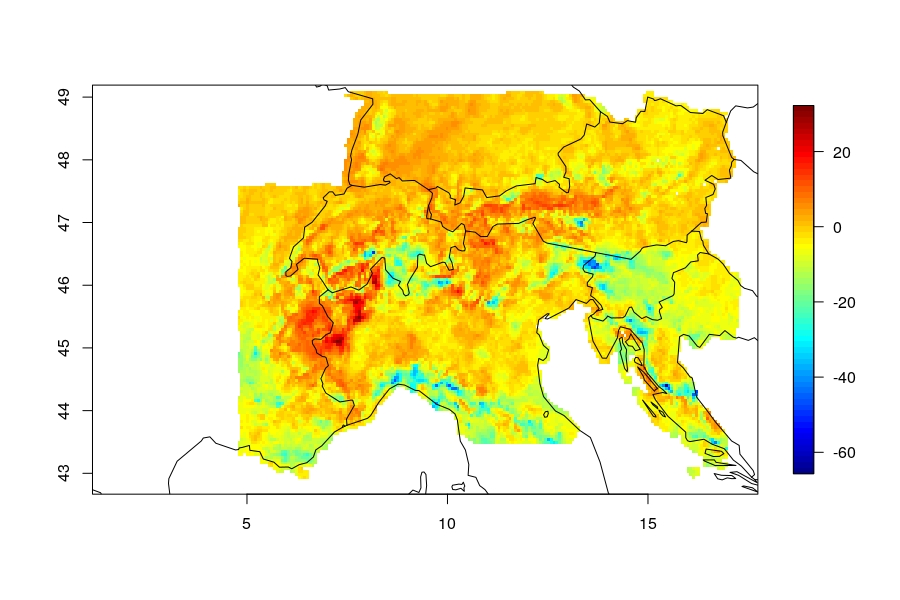
\includegraphics[width=\textwidth]{quantile_all/diff_q99_eval_eur11.jpeg}
		\caption{EUR-11, Evaluation}
	\end{subfigure}
	\begin{subfigure}{0.49\textwidth}
		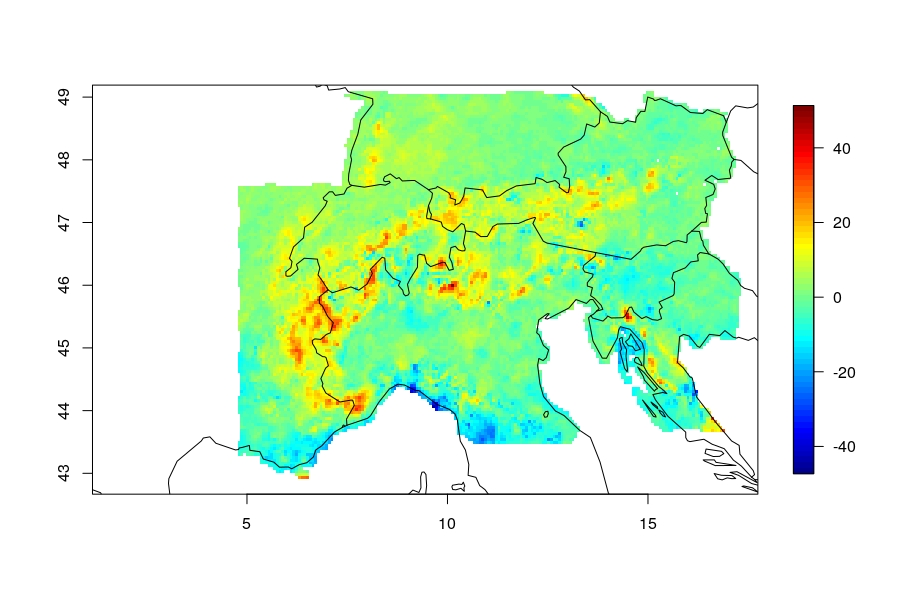
\includegraphics[width=\textwidth]{quantile_all/diff_q99_eval_alp3.jpeg}
		\caption{ALP-3, Evaluation}
	\end{subfigure}
	\caption{Geographische Verteilung der Abweichungen [mm/Tag] im 99. Quantil,für alle Jahre und für die 4 Datensätze. In Evaluation ALP-3 wurde, wie in Kapitel \ref{sec:diff_q99} beschrieben, ein Ausreißer-Bereich ausgeschnitten, für die unveränderte Darstellung siehe Abb. \ref{fig:quantile_eval_alp3}}
	\label{fig:quantile_all}
\end{figure}
\begin{figure}
	\begin{subfigure}{0.49\textwidth}
		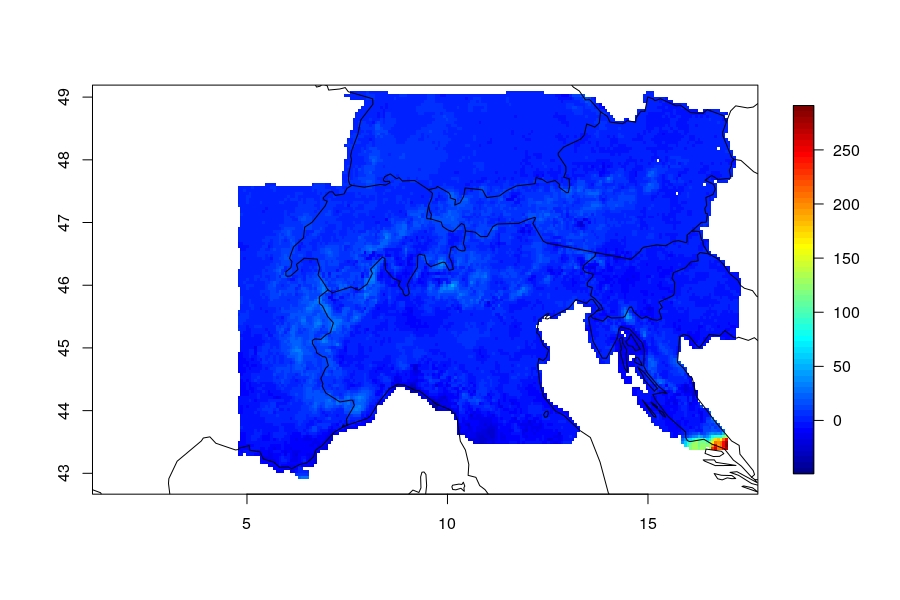
\includegraphics[width=\textwidth]{quantile_all/diff_q99_eval_alp3_uncropped.jpeg}
	\end{subfigure}
	\begin{subfigure}{0.49\textwidth}
		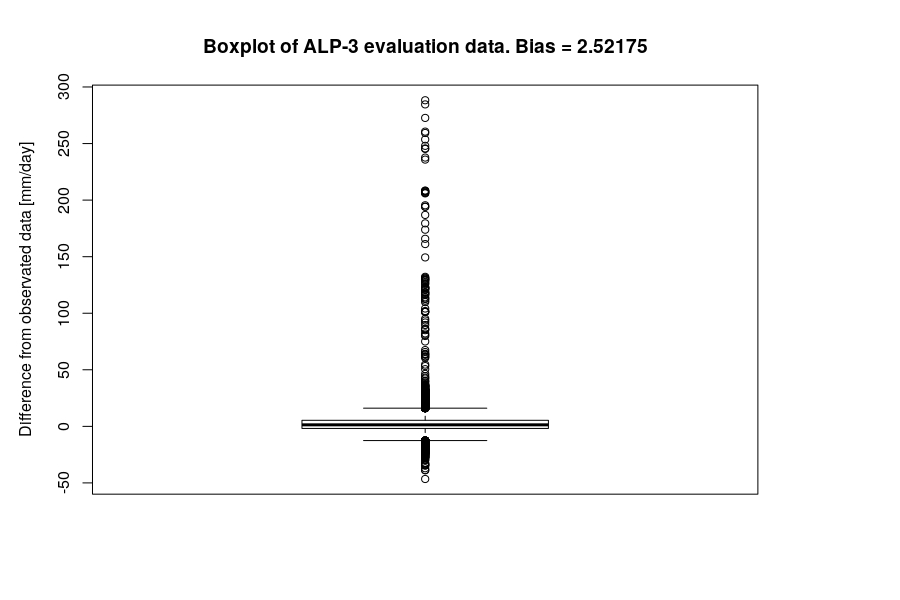
\includegraphics[width=\textwidth]{quantile_all/diff_q99_boxplot_eval_alp3_uncropped.jpeg}
	\end{subfigure}
	\caption{Abweichungen des Evaluation-ALP-3 Datensatzes im 99. Quantil mit klar ersichtlichem Ausreißer-Bereich im Süden Kroatiens.}
	\label{fig:quantile_eval_alp3}
\end{figure}

\section{Zusammenfassung}
In diesem Kapitel wurden die 99. Quantile und somit die modellierten Starkregenereignisse des gesamten Jahres mit den Beobachtungsdaten verglichen. Dadurch wurde ein guter Aufschluss darüber erlangt, wie die Starkregenereignisse im generellen durch die unterschiedlichen Datensätzen simuliert werden. Wie es scheint, herrscht eine relativ gute Übereinstimmung mit den tatsächlichen gemessenen Werten durch das Konvektion-erlaubende Modell CCLM5-0-9 über das gesamte Gebiet. Das Modell CCLM4-8-17, in welchem die Konvektion parametrisiert vorliegt, scheint die Abweichungen über das gesamte Gebiet vergleichsweise gleichbleibend groß zu sein. In den Abbildungen \ref{fig:quantile_all} erkennt man gut, dass manche Regionen besonders stark unterschätzte Starkregen-Ereignisse aufweisen: 
\begin{itemize}
	\item Der Bereich rund um Genua
	\item Das Grenzgebiet von Italien zur südlichen Schweiz
	\item Ein Bereich an der Slowenisch-Italienische Grenze
\end{itemize}
Diese Regionen wurden in ''Major flood disasters in Europe: 1950–2005'' \cite{barredo_major_2007} unter anderem als Regionen größerer Flutkatastrophen genannt. Das weißt darauf hin, dass diese Regionen durch die starken Wetterschwankungen besonders herausfordernd zu modellieren sind, bzw. das Feintunig noch nicht vollendet ist.

\section{R-Code}
\begin{lstlisting}[language = R]
	getQuantile <- function(list_allDays) # berechnen der Quantile
		qt_by_year<-raster()
		for(i in 1:10){
			dummy<-list_allDays[[i]]
			qt_by_year <- addLayer(qt_by_year, dummy)
		}
		qt_by_year<-calc(qt_by_year, fun=Q99)
		return(qt_by_year)
	}
	eval_eur11<-stackSim(getEUR11regridded_eval_pr(), varname="pr", factor=3600*24)# Modelldaten in eine Liste geben
	quantile_eval_eur11<-getQuantile(eval_eur11) # quantile berechnen
	dif_quantile_eval_eur11 <- overlay(quantile_eval_eur11, quantile_observations, fun=function(x,y){return((x - y))})# differenzen Berechnen
\end{lstlisting}
Ausschnitt des essenziellen Codes für einen Datensatz.